\subsubsection{Case Studies on DAPO-Qwen-32B}

% we use the same model as for the aime24 case to answer and verify.
We show how DAPO-Qwen-32B solves a question in AIME24 while Qwen2.5-32B arrives at the correct answer by guessing (see Appendix~\ref{supp_sec:aime24_case}).

\begin{questionbox}{ Question }
% \textbf{AIME24 Question No.14}
\textbf{AIME24 I Question No.14}

Let $ABCD$ be a tetrahedron such that $AB=CD= \sqrt{41}$, $AC=BD= \sqrt{80}$, and $BC=AD= \sqrt{89}$. There exists a point $I$ inside the tetrahedron such that the distances from $I$ to each of the faces of the tetrahedron are all equal. This distance can be written in the form $\frac{m \sqrt n}{p}$, where $m$, $n$, and $p$ are positive integers, $m$ and $p$ are relatively prime, and $n$ is not divisible by the square of any prime. Find $m+n+p$. 

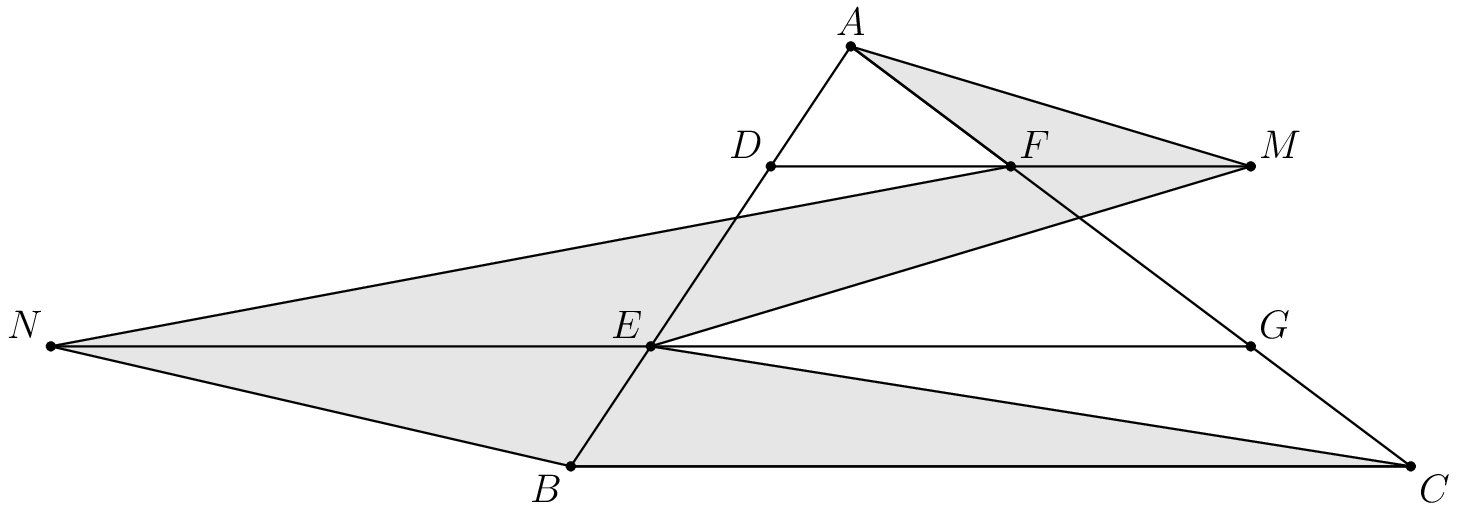
\includegraphics[height=8em]{figures/aime25-2.png}
\end{questionbox}

\begin{answerbox}{Qwen2.5-32B Answer}

To approach this math problem, we'll use the concept of the inradius of a tetrahedron. The inradius $r$ of a tetrahedron is the radius of the inscribed sphere that is tangent to all four faces of the tetrahedron. The formula for the inradius $r$ of a tetrahedron is given by

\[ r = \frac{3V}{A_1 + A_2 + A_3 + A_4}, \]

where $V$ is the volume of the tetrahedron and $A_1, A_2, A_3,$ and $A_4$ are the areas of the four faces.

First, we need to calculate the areas of the faces of the tetrahedron $ABCD$.

The faces of the tetrahedron are $\triangle ABC$, $\triangle ABD$, $\triangle ACD$, and $\triangle BCD$.

We will use Heron's formula to calculate the areas of these triangles.

For $\triangle ABC$, the sides are $AB = \sqrt{41}$, $BC = \sqrt{89}$, and $CA = \sqrt{80}$. The semi-perimeter $s_1$ of $\triangle ABC$ is:

\[ s_1 = \frac{AB + BC + CA}{2} = \frac{\sqrt{41} + \sqrt{89} + \sqrt{80}}{2}. \]

Using Heron's formula, the area of $\triangle ABC$ is

\[ \text{Area}_{\triangle ABC} = \sqrt{s_1 (s_1 - AB)(s_1 - BC)(s_1 - CA)}. \]

Let's simplify this step by step.

\[ s_1 = \frac{\sqrt{41} + \sqrt{89} + 4\sqrt{5}}{2}. \]

Now we calculate $(s_1 - AB)$, $(s_1 - BC)$, and $(s_1 - CA)$:

\[ s_1 - AB = \frac{\sqrt{41} + \sqrt{89} + 4\sqrt{5}}{2} - \sqrt{41} = \frac{\sqrt{89} + 4 \sqrt{5} - \sqrt{41}}{2}, \]

\[ s_1 - BC = \frac{\sqrt{41} + \sqrt{89} + 4 \sqrt{5}}{2} - \sqrt{89} = \frac{\sqrt{41} + 4 \sqrt{5} - \sqrt{89}}{2}, \]

and

\[ s_1 - CA = \frac{\sqrt{41} + \sqrt{89} + 4 \sqrt{5}}{2} - 4 \sqrt{5} = \frac{\sqrt{41} + \sqrt{89} - 4 \sqrt{5}}{2}. \]

Thus the area of $\triangle ABC$ is:

\[ \text{Area}_{\triangle ABC} = \]
\[ \sqrt{\left(\frac{\sqrt{41} + \sqrt{89} + 4 \sqrt{5}}{2}\right) \left(\frac{\sqrt{89} + 4 \sqrt{5} - \sqrt{41}}{2}\right) \left(\frac{\sqrt{41} + 4 \sqrt{5} - \sqrt{89}}{2}\right) \left(\frac{\sqrt{41} + \sqrt{89} - 4 \sqrt{5}}{2}\right)}. \]

This expression looks complicated, so let's calculate the areas of the other triangles and see if we can find a simpler approach.

Now, we calculate the area of $\triangle ABD$. The sides are $AB = \sqrt{41}$, $BD = \sqrt{80}$, and $DA = \sqrt{89}$. The semi-perimeter $s_2$ of $\triangle ABD$ is:

\[ s_2 = \frac{\sqrt{41} + \sqrt{80} + \sqrt{89}}{2} = \frac{\sqrt{41} + 4 \sqrt{5} + \sqrt{89}}{2}. \]

Using Heron's formula, the area of $\triangle ABD$ is

\[ \text{Area}_{\triangle ABD} = \sqrt{s_2 (s_2 - AB)(s_2 - BD)(s_2 - DA)}. \]

We calculate each term:

\[ s_2 - AB = \frac{\sqrt{41} + 4 \sqrt{5} + \sqrt{89}}{2} - \sqrt{41} = \frac{4 \sqrt{5} + \sqrt{89} - \sqrt{41}}{2}, \]

\[ s_2 - BD = \frac{\sqrt{41} + 4 \sqrt{5} + \sqrt{89}}{2} - 4 \sqrt{5} = \frac{\sqrt{41} + \sqrt{89} - 4 \sqrt{5}}{2}, \]

\end{answerbox}

and

\[ s_2 - DA = \frac{\sqrt{41} + 4 \sqrt{5} + \sqrt{89}}{2} - \sqrt{89} = \frac{\sqrt{41} + 4 \sqrt{5} - \sqrt{89}}{2}. \]

Thus the area of $\triangle ABD$ is:

\[ \text{Area}_{\triangle ABD} = \sqrt{\left(\frac{\sqrt{41} + 4 \sqrt{5} + \sqrt{89}}{2}\right) \left(\frac{4 \sqrt{5} + \sqrt{89} - \sqrt{41}}{2}\right) \left(\frac{\sqrt{41} + \sqrt{89} - 4 \sqrt{5}}{2}\right) \left(\frac{\sqrt{41} + 4 \sqrt{5} - \sqrt{89}}{2}\right)}. \]

Notice that the expressions for the areas of $\triangle ABC$ and $\triangle ABD$ look very similar. Let's calculate the area of $\triangle ACD$ next. The sides are $AC = \sqrt{80} = 4\sqrt{5}$, $CD = \sqrt{41}$, and $DA = \sqrt{89}$. The semi-perimeter $s_3$ is:

\[ s_3 = \frac{\sqrt{80} + \sqrt{41} + \sqrt{89}}{2} = \frac{4 \sqrt{5} + \sqrt{41} + \sqrt{89}}{2}. \]

Using Heron's formula, the area of $\triangle ACD$ is

\[ \text{Area}_{\triangle ACD} = \sqrt{s_3 (s_3 - AC)(s_3 - CD)(s_3 - DA)}. \]

We calculate each term:

\[ s_3 - AC = \frac{4 \sqrt{5} + \sqrt{41} + \sqrt{89}}{2} - 4 \sqrt{5} = \frac{\sqrt{41} + \sqrt{89} - 4 \sqrt{5}}{2}, \]

\[ s_3 - CD = \frac{4 \sqrt{5} + \sqrt{41} + \sqrt{89}}{2} - \sqrt{41} = \frac{4 \sqrt{5} + \sqrt{89} - \sqrt{41}}{2}, \]

and

\[ s_3 - DA = \frac{4 \sqrt{5} + \sqrt{41} + \sqrt{89}}{2} - \sqrt{89} = \frac{4 \sqrt{5} + \sqrt{41} - \sqrt{89}}{2}. \]

Thus the area of $\triangle ACD$ is

\[ \text{Area}_{\triangle ACD} = \sqrt{\left(\frac{4 \sqrt{5} + \sqrt{41} + \sqrt{89}}{2}\right) \left(\frac{\sqrt{41} + \sqrt{89} - 4 \sqrt{5}}{2}\right) \left(\frac{4 \sqrt{5} + \sqrt{89} - \sqrt{41}}{2}\right) \left(\frac{4 \sqrt{5} + \sqrt{41} - \sqrt{89}}{2}\right)}. \]

Finally, we calculate the area of $\triangle BCD$. The sides are $BC = \sqrt{89}$, $CD = \sqrt{41}$, and $BD = \sqrt{80} = 4 \sqrt{5}$. The semi-perimeter $s_4$ is

\[ s_4 = \frac{\sqrt{89} + \sqrt{41} + 4 \sqrt{5}}{2}. \]

Using Heron's formula, the area of $\triangle BCD$ is

\[ \text{Area}_{\triangle BCD} = \sqrt{s_4 (s_4 - BC)(s_4 - CD)(s_4 - BD)}. \]

We calculate each term:

\[ s_4 - BC = \frac{\sqrt{89} + \sqrt{41} + 4 \sqrt{5}}{2} - \sqrt{89} = \frac{\sqrt{41} + 4 \sqrt{5} - \sqrt{89}}{2}, \]

\[ s_4 - CD = \frac{\sqrt{89} + \sqrt{41} + 4 \sqrt{5}}{2} - \sqrt{41} = \frac{\sqrt{89} + 4 \sqrt{5} - \sqrt{41}}{2}, \]

and

\[ s_4 - BD = \frac{\sqrt{89} + \sqrt{41} + 4 \sqrt{5}}{2} - 4 \sqrt{5} = \frac{\sqrt{89} + \sqrt{41} - 4 \sqrt{5}}{2}. \]

Thus the area of $\triangle BCD$ is

\[ \text{Area}_{\triangle BCD} = \sqrt{\left(\frac{\sqrt{89} + \sqrt{41} + 4 \sqrt{5}}{2}\right) \left(\frac{\sqrt{41} + 4 \sqrt{5} - \sqrt{89}}{2}\right) \left(\frac{\sqrt{89} + 4 \sqrt{5} - \sqrt{41}}{2}\right) \left(\frac{\sqrt{89} + \sqrt{41} - 4 \sqrt{5}}{2}\right)}. \]

Notice that the expressions for the areas of $\triangle ABC$, $\triangle ABD$, $\triangle ACD$, and $\triangle BCD$ are identical. Therefore, all four faces have the same area.

Let's denote this common area by $A$. We have

\[ A = \sqrt{\left(\frac{\sqrt{41} + \sqrt{89} + 4 \sqrt{5}}{2}\right) \left(\frac{\sqrt{89} + 4 \sqrt{5} - \sqrt{41}}{2}\right) \left(\frac{\sqrt{41} + 4 \sqrt{5} - \sqrt{89}}{2}\right) \left(\frac{\sqrt{41} + \sqrt{89} - 4 \sqrt{5}}{2}\right)}. \]

To simplify this expression, we use the identity for the area of a triangle given its sides $a$, $b$, and $c$: 

\[ \text{Area} = \frac{1}{4} \sqrt{(a^2 + b^2 + c^2)^2 - 2(a^4 + b^4 + c^4)}. \]

Let's apply this to $\triangle ABC$ with sides $a = \sqrt{41}$, $b = \sqrt{89}$, and $c = \sqrt{80} = 4\sqrt{5}$.

First, we calculate $a^2$, $b^2$, and $c^2$:

\[ a^2 = 41, \]
\[ b^2 = 89, \]
\[ c^2 = 80. \]

Then we compute $(a^2 + b^2 + c^2)^2$:

\[ a^2 + b^2 + c^2 = 41 + 89 + 80 = 210, \]

so

\[ (a^2 + b^2 + c^2)^2 = 210^2 = 44100. \]

Next, we compute $a^4$, $b^4$, and $c^4$:

\[ a^4 = (41)^2 = 1681, \]
\[ b^4 = (89)^2 = 7921, \]
\[ c^4 = (80)^2 = 6400. \]

Then we compute $a^4 + b^4 + c^4$:

\[ a^4 + b^4 + c^4 = 1681 + 7921 + 6400 = 16002. \]

Now we use the identity for the area:

\[ \text{Area}_{\triangle ABC} = \frac{1}{4} \sqrt{(a^2 + b^2 + c^2)^2 - 2(a^4 + b^4 + c^4)} = \frac{1}{4} \sqrt{44100 - 2 \cdot 16002} = \frac{1}{4} \sqrt{44100 - 32004} = \frac{1}{4} \sqrt{12096} = \frac{1}{4} \times \sqrt{12096} = \frac{1}{4} \times \sqrt{144 \times 84} = \frac{1}{4} \times 12 \sqrt{84} = \frac{1}{4} \times 12 \sqrt{4 \cdot 21} = \frac{1}{4} \times 12 \times 2 \sqrt{21} = \frac{1}{4} \times 24 \sqrt{21} = 6 \sqrt{21}. \]

So the area of $\triangle ABC$ is $6 \sqrt{21}$. Since all the faces have the same area, each face has area $6 \sqrt{21}$.

The total surface area $A_{\text{total}}$ of the tetrahedron is therefore 

\[ A_{\text{total}} = 4 \times 6 \sqrt{21} = 24 \sqrt{21}. \]

Next, we need to find the volume $V$ of the tetrahedron $ABCD$.

To find the volume, we can use the coordinates of the vertices and the formula for the volume of a tetrahedron given its vertices.

Let's place the vertices of the tetrahedron in a coordinate system to make the calculations easier.

Let's set the coordinates as follows:

- $A = (0, 0, 0)$,
- $B = (\sqrt{41}, 0, 0)$ since $AB = \sqrt{41}$.

Now we need to find the coordinates of $D$ and $C$ such that the given distances are satisfied.

Let $D = (d_1, d_2, 0)$ and $C = (c_1, c_2, c_3)$.

We have the following distance conditions:

1. $BD = \sqrt{(d_1 - \sqrt{41})^2 + d_2^2} = \sqrt{80}$,
2. $AD = \sqrt{d_1^2 + d_2^2} = \sqrt{89}$,
3. $AC = \sqrt{c_1^2 + c_2^2 + c_3^2} = \sqrt{80}$,
4. $BC = \sqrt{(c_1 - \sqrt{41})^2 + c_2^2 + c_3^2} = \sqrt{89}$,
5. $CD = \sqrt{(c_1 - d_1)^2 + (c_2 - d_2)^2 + c_3^2} = \sqrt{41}$.

From condition 2 ($AD = \sqrt{89}$), we get

\[ d_1^2 + d_2^2 = 89. \tag*{(i)} \]

From condition 1 ($BD = \sqrt{80}$), we get

\[ (d_1 - \sqrt{41})^2 + d_2^2 = 80. \tag*{(ii)} \]

Expanding (ii), we obtain

\[ d_1^2 - 2 \sqrt{41} d_1 + 41 + d_2^2 = 80. \]

Using equation (i) ($d_1^2 + d_2^2 = 89$), we can substitute $d_1^2 + d_2^2$ in the above equation to get

\[ 89 - 2 \sqrt{41} d_1 + 41 = 80. \]

This simplifies to

\[ 130 - 2 \sqrt{41} d_1 = 80, \]

so

\[ 2 \sqrt{41} d_1 = 50, \]

and thus

\[ d_1 = \frac{50}{2 \sqrt{41}} = \frac{25}{\sqrt{41}} = \frac{25 \sqrt{41}}{41}. \]

Substitute $d_1 = \frac{25 \sqrt{41}}{41}$ into equation (i):

\[ \left(\frac{25 \sqrt{41}}{41}\right)^2 + d_2^2 = 89. \]

This simplifies to

\[ \frac{625 \times 41}{1681} + d_2^2 = 89, \]

or

\[ \frac{625}{41} + d_2^2 = 89. \]

Rearranging gives us

\[ d_2^2 = 89 - \frac{625}{41} = \frac{3649 - 625}{41} = \frac{3024}{41}. \]

Thus

\[ d_2 = \sqrt{\frac{3024}{41}} = \frac{\sqrt{3024}}{\sqrt{41}} = \frac{12 \sqrt{21}}{\sqrt{41}} = \frac{12 \sqrt{861}}{41}. \]

Therefore, the coordinates of $D$ are $\left(\frac{25 \sqrt{41}}{41}, \frac{12 \sqrt{861}}{41}, 0\right)$.

Now we need to find the coordinates of $C = (c_1, c_2, c_3)$. We have the following conditions from the distances:

1. $AC = \sqrt{c_1^2 + c_2^2 + c_3^2} = \sqrt{80}$, which simplifies to

\[ c_1^2 + c_2^2 + c_3^2 = 80, \tag*{(iii)} \]

2. $BC = \sqrt{(c_1 - \sqrt{41})^2 + c_2^2 + c_3^2} = \sqrt{89}$, which expands to

\[ (c_1 - \sqrt{41})^2 + c_2^2 + c_3^2 = 89. \tag*{(iv)} \]

Expanding (iv), we get

\[ c_1^2 - 2 \sqrt{41} c_1 + 41 + c_2^2 + c_3^2 = 89. \]

Using equation (iii) ($c_1^2 + c_2^2 + c_3^2 = 80$), we substitute $c_1^2 + c_2^2 + c_3^2$ into the above equation to obtain

\[ 80 - 2 \sqrt{41} c_1 + 41 = 89. \]

This simplifies to

\[ 121 - 2 \sqrt{41} c_1 = 89, \]

so

\[ 2 \sqrt{41} c_1 = 32, \]

and thus

\[ c_1 = \frac{32}{2 \sqrt{41}} = \frac{16}{\sqrt{41}} = \frac{16 \sqrt{41}}{41}. \tag*{(v)} \]

Now we use condition (iii) ($c_1^2 + c_2^2 + c_3^2 = 80$) and substitute $c_1 = \frac{16 \sqrt{41}}{41}$ into it:

\[ \left(\frac{16 \sqrt{41}}{41}\right)^2 + c_2^2 + c_3^2 = 80. \]

This simplifies to

\[ \frac{256 \times 41}{1681} + c_2^2 + c_3^2 = 80, \]

or

\[ \frac{256}{41} + c_2^2 + c_3^2 = 80. \]

Rewriting this, we get

\[ c_2^2 + c_3^2 = 80 - \frac{256}{41} = \frac{3280 - 256}{41} = \frac{3024}{41}. \tag*{(vi)} \]

Finally, we use the condition for the distance $CD = \sqrt{(c_1 - d_1)^2 + (c_2 - d_2)^2 + c_3^2} = \sqrt{41}$. Using the values we have for $c_1$ and $d_1$, we get

\[ c_1 - d_1 = \frac{16 \sqrt{41}}{41} - \frac{25 \sqrt{41}}{41} = \frac{-9 \sqrt{41}}{41}, \]

so 

\[ (c_1 - d_1)^2 = \left(\frac{-9 \sqrt{41}}{41}\right)^2 = \frac{81 \cdot 41}{1681} = \frac{81}{41}. \]

Now, using the expression for $CD$, we get

\[ CD = \sqrt{(c_1 - d_1)^2 + (c_2 - d_2)^2 + c_3^2} = \sqrt{\frac{81}{41} + (c_2 - d_2)^2 + c_3^2} = \sqrt{41}. \]

Thus,

\[ \frac{81}{41} + (c_2 - d_2)^2 + c_3^2 = 41. \]

Rewriting this, we have

\[ (c_2 - d_2)^2 + c_3^2 = 41 - \frac{81}{41} = \frac{1681 - 81}{41} = \frac{1600}{41}. \tag*{(vii)} \]

From equation (vi), we know that $c_2^2 + c_3^2 = \frac{3024}{41}$. Using this in equation (vii), we get

\[ (c_2 - d_2)^2 + c_3^2 = \frac{1600}{41}, \]

and expanding $(c_2 - d_2)^2$, we have

\[ (c_2 - d_2)^2 = c_2^2 - 2 c_2 d_2 + d_2^2. \]

Thus,

\[ c_2^2 - 2 c_2 d_2 + d_2^2 + c_3^2 = \frac{1600}{41}. \]

Using $c_2^2 + c_3^2 = \frac{3024}{41}$ from equation (vi), we can substitute to get

\[ \frac{3024}{41} - 2 c_2 d_2 + d_2^2 = \frac{1600}{41}. \]

Rearranging gives

\[ \frac{3024}{41} - \frac{1600}{41} = 2 c_2 d_2 - d_2^2, \]

or

\[ \frac{1424}{41} = 2 c_2 d_2 - d_2^2. \]

Rewriting this, we obtain

\[ 2 c_2 d_2 - d_2^2 = \frac{1424}{41}. \]

From earlier, we have $d_2 = \frac{12 \sqrt{861}}{41}$. Substitute this into the equation:

\[ 2 c_2 \left(\frac{12 \sqrt{861}}{41}\right) - \left(\frac{12 \sqrt{861}}{41}\right)^2 = \frac{1424}{41}. \]

Simplifying the first term, we get

\[ 2 c_2 \left(\frac{12 \sqrt{861}}{41}\right) = \frac{24 c_2 \sqrt{861}}{41}, \]

and simplifying the second term, we have

\[ \left(\frac{12 \sqrt{861}}{41}\right)^2 = \frac{144 \cdot 861}{1681} = \frac{144 \cdot 861}{41^2} = \frac{144 \cdot 861}{1681}. \]

To simplify $\frac{144 \cdot 861}{1681}$, note that $861 = 21 \times 41$, so

\[ \frac{144 \cdot 861}{1681} = \frac{144 \cdot (21 \times 41)}{41^2} = \frac{144 \cdot 21 \times 41}{41^2} = \frac{144 \cdot 21}{41}. \]

Thus the equation becomes

\[ \frac{24 c_2 \sqrt{861}}{41} - \frac{144 \cdot 21}{41} = \frac{1424}{41}. \]

Multiplying through by $41$, we get

\[ 24 c_2 \sqrt{861} - 144 \cdot 21 = 1424. \]

Simplifying $144 \cdot 21$, we get

\[ 144 \times 21 = 144 \times 20 + 144 \times 1 = 2880 + 144 = 3024. \]

Thus the equation becomes

\[ 24 c_2 \sqrt{861} - 3024 = 1424. \]

Rearranging gives

\[ 24 c_2 \sqrt{861} = 4448. \]

Dividing both sides by 24, we get

\[ c_2 \sqrt{861} = \frac{4448}{24} = \frac{2224}{12} = \frac{1112}{6} = \frac{556}{3}. \]

Therefore,

\[ c_2 = \frac{556}{3 \sqrt{861}} = \frac{556 \sqrt{861}}{3 \times 861} = \frac{556 \sqrt{861}}{2583}. \]

Now we need to find $c_3$. From equation (vi), we have

\[ c_2^2 + c_3^2 = \frac{3024}{41}. \]

Substitute $c_2 = \frac{556 \sqrt{861}}{2583}$ into this equation. First, calculate $c_2^2$:

\[ c_2^2 = \left(\frac{556 \sqrt{861}}{2583}\right)^2 = \frac{(556)^2 \times 861}{2583^2}. \]

We need to simplify $(556)^2$ and $2583^2$.

$(556)^2 = 309136,$

and 

$2583 = 3 \times 861,$

so 

$2583^2 = (3 \times 861)^2 = 9 \times 861^2.$

Thus 

\[ c_2^2 = \frac{309136 \times 861}{9 \times 861^2} = \frac{309136}{9 \times 861}. \]

Now substitute $c_2^2$ back into the equation $c_2^2 + c_3^2 = \frac{3024}{41}$:

\[ \frac{309136}{9 \times 861} + c_3^2 = \frac{3024}{41}. \]

Rewrite $9 \times 861$:

\[ 9 \times 861 = 7749. \]

Thus the equation becomes

\[ \frac{309136}{7749} + c_3^2 = \frac{3024}{41}. \]

Rewriting $\frac{309136}{7749}$ over a common denominator with $\frac{3024}{41}$ requires some manipulation. Let's first get a common denominator for both fractions.

The common denominator is $7749 \times 41$.

Rewrite $\frac{309136}{7749}$:

\[ \frac{309136}{7749}. \]

Rewrite $\frac{3024}{41}$ with the common denominator:

\[ \frac{3024}{41} = \frac{3024 \times 7749}{41 \times 7749}. \]

Now our equation becomes

\[ \frac{309136}{7749} + c_3^2 = \frac{3024 \times 7749}{41 \times 7749}. \]

Rewriting the entire equation with the common denominator $7749 \times 41$, we get

\[ \frac{309136 \times 41}{7749 \times 41} + c_3^2 = \frac{3024 \times 7749}{41 \times 7749}. \]

So 

\[ c_3^2 = \frac{3024 \times 7749}{41 \times 7749} - \frac{309136 \times 41}{7749 \times 41} = \frac{3024 \times 7749 - 309136 \times 41}{41 \times 7749}. \]

To simplify the numerator $3024 \times 7749 - 309136 \times 41$, we can factor out common terms if possible.

Notice that 

\[ 3024 \times 7749 = 3024 \times (7749), \]

and

\[ 309136 \times 41. \]

Let's simplify each term separately.

First, calculate $3024 \times 7749$:

\[ 3024 \times 7749 = 3024 \times (7700 + 49). \]

Using the distributive property, 

\[ 3024 \times 7700 + 3024 \times 49. \]

Now, calculate $3024 \times 7700$:

\[ 3024 \times 7700 = 3024 \times 77 \times 100. \]

Calculate $3024 \times 77$:

\[ 3024 \times 77 = 3024 \times (70 + 7) = 3024 \times 70 + 3024 \times 7. \]

Calculate $3024 \times 70$:

\[ 3024 \times 70 = 3024 \times 7 \times 10 = 21168 \times 10 = 211680. \]

Calculate $3024 \times 7$:

\[ 3024 \times 7 = 21168. \]

Now add them together:

\[ 3024 \times 77 = 211680 + 21168 = 232848. \]

So 

\[ 3024 \times 7700 = 232848 \times 100 = 23284800. \]

Next, calculate $3024 \times 49$:

\[ 3024 \times 49 = 3024 \times (50 - 1) = 3024 \times 50 - 3024 \times 1. \]

Calculate $3024 \times 50$:

\[ 3024 \times 50 = 151200. \]

And 

\[ 3024 \times 1 = 3024. \]

So 

\[ 3024 \times 49 = 151200 - 3024 = 148176. \]

Now add the two results for $3024 \times 7749$:

\[ 3024 \times 7749 = 23284800 + 148176 = 23432976. \]

Now we calculate $309136 \times 41$.

Use the distributive property:

\[ 309136 \times 41 = 309136 \times 40 + 309136 \times 1. \]

Calculate $309136 \times 40$:

\[ 309136 \times 40 = 12365440. \]

And

\[ 309136 \times 1 = 309136. \]

So 

\[ 309136 \times 41 = 12365440 + 309136 = 12674576. \]

Now we subtract the two results:

\[ 3024 \times 7749 - 309136 \times 41 = 23432976 - 12674576 = 10758400. \]

Thus the numerator simplifies to $10758400$.

So 

\[ c_3^2 = \frac{10758400}{41 \times 7749}. \]

We can simplify this further. Notice that

\[ 41 \times 7749 = 41 \times (7749). \]

Let's simplify $7749$:

\[ 7749 \div 3 = 2583, \]
\[ 2583 \div 3 = 861, \]
and 

\[ 861 \div 3 = 287. \]

So $7749 = 3^3 \times 287.$

Now we have 

\[ 41 \times 7749 = 41 \times 3^3 \times 287. \]

Next, simplify the fraction $\frac{10758400}{41 \times 7749}$:

We need to factorize $10758400$.

Notice that 

\[ 10758400 \div 100 = 107584, \]

so 

\[ 10758400 = 107584 \times 100. \]

Now, factorize $100$:

\[ 100 = 2^2 \times 5^2. \]

So 

\[ 10758400 = 107584 \times 2^2 \times 5^2. \]

Next, factorize $107584$:

\[ 107584 \div 2 = 53792, \]
\[ 53792 \div 2 = 26896, \]
\[ 26896 \div 2 = 13448, \]
\[ 13448 \div 2 = 6724, \]
\[ 6724 \div 2 = 3362, \]
\[ 3362 \div 2 = 1681, \]
and 

\[ 1681 = 41^2. \]

Thus the prime factorization of $107584$ is 

\[ 107584 = 2^6 \times 1681 = 2^6 \times 41^2. \]

So the prime factorization of $10758400$ is

\[ 10758400 = 2^6 \times 41^2 \times 2^2 \times 5^2 = 2^8 \times 41^2 \times 5^2. \]

Now we can rewrite the fraction $\frac{10758400}{41 \times 7749}$ using the prime factorizations:

\[ \frac{10758400}{41 \times 7749} = \frac{2^8 \times 41^2 \times 5^2}{41 \times 7749}. \]

Cancel one $41$ from the numerator and the denominator:

\[ \frac{2^8 \times 41 \times 5^2}{7749}. \]

Recall that $7749 = 3^3 \times 287.$

Thus the fraction becomes

\[ \frac{2^8 \times 41 \times 5^2}{3^3 \times 287}. \]

To simplify this further, we need to check if 287 can be factored further. We find that

\[ 287 \div 7 = 41. \]

So 

\[ 287 = 7 \times 41. \]

Thus 

\[ 7749 = 3^3 \times 287 = 3^3 \times 7 \times 41. \]

Substitute this back into the fraction:

\[ \frac{2^8 \times 41 \times 5^2}{3^3 \times 7 \times 41}. \]

Cancel the $41$ from the numerator and the denominator:

\[ \frac{2^8 \times 5^2}{3^3 \times 7} = \frac{256 \times 25}{27 \times 7} = \frac{6400}{189}. \]

Therefore,

\[ c_3^2 = \frac{6400}{189}. \]

Taking the square root gives us

\[ c_3 = \sqrt{\frac{6400}{189}} = \frac{\sqrt{6400}}{\sqrt{189}} = \frac{80}{\sqrt{189}} = \frac{80 \sqrt{189}}{189}. \]

Since $\sqrt{189} = \sqrt{9 \times 21} = 3 \sqrt{21},$

we have

\[ c_3 = \frac{80 \cdot 3 \sqrt{21}}{189} = \frac{240 \sqrt{21}}{189} = \frac{80 \sqrt{21}}{63}. \]

So the coordinates for $C$ are $\left(\frac{16 \sqrt{41}}{41}, \frac{556 \sqrt{861}}{2583}, \frac{80 \sqrt{21}}{63}\right).$

Now that we have the coordinates for $A$, $B$, $D$, and $C$, we can use the formula for the volume of a tetrahedron given vertices $A(0,0,0)$, $B(\sqrt{41},0,0)$, $D \left(\frac{25 \sqrt{41}}{41}, \frac{12 \sqrt{861}}{41}, 0\right),$ and $C \left(\frac{16 \sqrt{41}}{41}, \frac{556 \sqrt{861}}{2583}, \frac{80 \sqrt{21}}{63}\right).$

The volume $V$ of the tetrahedron with vertices $A(0,0,0),$ $B(x_1, y_1, z_1),$ $D(x_2, y_2, z_2),$ and $C(x_3, y_3, z_3)$ is given by

\[ V = \frac{1}{6} \left| \det \begin{vmatrix}
x_1 & y_1 & z_1 \\ 
x_2 & y_2 & z_2 \\ 
x_3 & y_3 & z_3 
\end{vmatrix} \right|. \]

Substitute in the coordinates for $B$, $D$, and $C$:

$B = \left(\sqrt{41}, 0, 0\right),$

$D = \left(\frac{25 \sqrt{41}}{41}, \frac{12 \sqrt{861}}{41}, 0\right),$

and 

$C = \left(\frac{16 \sqrt{41}}{41}, \frac{556 \sqrt{861}}{2583}, \frac{80 \sqrt{21}}{63}\right).$

The determinant we need to compute is

\[ \det \begin{vmatrix}
\sqrt{41} & 0 & 0 \\ 
\frac{25 \sqrt{41}}{41} & \frac{12 \sqrt{861}}{41} & 0 \\ 
\frac{16 \sqrt{41}}{41} & \frac{556 \sqrt{861}}{2583} & \frac{80 \sqrt{21}}{63}
\end{vmatrix}. \]

We can expand this determinant along the first row:

\[ \det = \sqrt{41} \begin{vmatrix} \frac{12 \sqrt{861}}{41} & 0 \\ \frac{556 \sqrt{861}}{2583} & \frac{80 \sqrt{21}}{63} \end{vmatrix} - 0 + 0. \]

So we only need to compute the $2 \times 2$ determinant:

\[ \begin{vmatrix} \frac{12 \sqrt{861}}{41} & 0 \\ \frac{556 \sqrt{861}}{2583} & \frac{80 \sqrt{21}}{63} \end{vmatrix}. \]

The determinant of this $2 \times 2$ matrix is

\[ \left(\frac{12 \sqrt{861}}{41}\right) \left(\frac{80 \sqrt{21}}{63}\right) - \left(0 \cdot \frac{556 \sqrt{861}}{2583}\right) = \frac{12 \sqrt{861}}{41} \cdot \frac{80 \sqrt{21}}{63}. \]

Now, simplify this expression:

\[ \frac{12 \sqrt{861}}{41} \cdot \frac{80 \sqrt{21}}{63} = \frac{12 \times 80 \times \sqrt{861} \times \sqrt{21}}{41 \times 63}. \]

Combine the constants and the square roots:

\[ \frac{960 \sqrt{861 \times 21}}{41 \times 63}. \]

Recall that $861 = 21 \times 41,$ so

\[ 861 \times 21 = (21 \times 41) \times 21 = 21^2 \times 41. \]

Thus 

\[ \sqrt{861 \times 21} = \sqrt{21^2 \times 41} = 21 \sqrt{41}. \]

Substitute this back into the expression:

\[ \frac{960 \times 21 \sqrt{41}}{41 \times 63}. \]

Now, simplify the fraction:

\[ \frac{960 \times 21 \sqrt{41}}{41 \times 63}. \]

Notice that $21$ in the numerator and $63$ in the denominator can be simplified since $63 = 3 \times 21$. Thus the fraction becomes

\[ \frac{960 \times 21 \sqrt{41}}{41 \times 63} = \frac{960 \times 21 \sqrt{41}}{41 \times 3 \times 21} = \frac{960 \sqrt{41}}{41 \times 3} = \frac{960 \sqrt{41}}{123}. \]

Simplifying $\frac{960}{123},$ we get

\[ \frac{960 \div 3}{123 \div 3} = \frac{320}{41}. \]

Thus the determinant is 

\[ \frac{320 \sqrt{41}}{41}. \]

Now, multiply this result by $\sqrt{41}$ from the expansion of the $3 \times 3$ determinant:

\[ \sqrt{41} \cdot \frac{320 \sqrt{41}}{41} = \frac{320 \times 41}{41} = 320. \]

Therefore, the volume $V$ is

\[ V = \frac{1}{6} \left| 320 \right| = \frac{320}{6} = \frac{160}{3}. \]

Now we have the volume $V = \frac{160}{3}$ and the total surface area $A_{\text{total}} = 24 \sqrt{21}$.

Using the formula for the inradius $r$:

\[ r = \frac{3V}{A_{\text{total}}} = \frac{3 \cdot \frac{160}{3}}{24 \sqrt{21}} = \frac{160}{24 \sqrt{21}} = \frac{20}{3 \sqrt{21}}. \]

Rationalize the denominator:

\[ r = \frac{20}{3 \sqrt{21}} \cdot \frac{\sqrt{21}}{\sqrt{21}} = \frac{20 \sqrt{21}}{3 \times 21} = \frac{20 \sqrt{21}}{63}. \]

Thus the inradius is $\frac{20 \sqrt{21}}{63}$. This is in the form $\frac{m \sqrt{n}}{p}$ where $m = 20$, $n = 21$, and $p = 63$. 

Therefore, $m + n + p = 20 + 21 + 63 = 104$.

Answer: 104


